\documentclass{article}

% if you need to pass options to natbib, use, e.g.:
% \PassOptionsToPackage{numbers, compress}{natbib}
% before loading nips_2018

% ready for submission
\usepackage{nips_2018}

% to compile a preprint version, e.g., for submission to arXiv, add
% add the [preprint] option:
% \usepackage[preprint]{nips_2018}

% to compile a camera-ready version, add the [final] option, e.g.:
% \usepackage[final]{nips_2018}

% to avoid loading the natbib package, add option nonatbib:
% \usepackage[nonatbib]{nips_2018}

\usepackage[utf8]{inputenc} % allow utf-8 input
\usepackage[T1]{fontenc}    % use 8-bit T1 fonts
\usepackage{hyperref}       % hyperlinks
\usepackage{url}            % simple URL typesetting
\usepackage{booktabs}       % professional-quality tables
\usepackage{amsfonts}       % blackboard math symbols
\usepackage{amsmath}
\usepackage{amssymb}
\usepackage{nicefrac}       % compact symbols for 1/2, etc.
\usepackage{microtype}      % microtypography
\usepackage{algorithm}
\usepackage{graphicx}
\usepackage{multirow}
\usepackage{comment}
\usepackage[bottom]{footmisc}
%\usepackage{subfig}
\usepackage{subcaption}
\usepackage[usenames,dvipsnames]{color}
\usepackage{bm}
\usepackage[font=footnotesize]{caption}
\usepackage{appendix}
\usepackage[nameinlink,noabbrev]{cleveref}
\crefname{appsec}{appendix}{appendices}
\usepackage{amsmath}
\usepackage[noend]{algpseudocode}
\usepackage{etoolbox}\AtBeginEnvironment{algorithmic}{\footnotesize}

\title{Target Encoding Networks}

% The \author macro works with any number of authors. There are two
% commands used to separate the names and addresses of multiple
% authors: \And and \AND.
%
% Using \And between authors leaves it to LaTeX to determine where to
% break the lines. Using \AND forces a line break at that point. So,
% if LaTeX puts 3 of 4 authors names on the first line, and the last
% on the second line, try using \AND instead of \And before the third
% author name.

\author{
  David S.~Hippocampus\thanks{Use footnote for providing further
  information about author (webpage, alternative
  address)---\emph{not} for acknowledging funding agencies.} \\
  Department of Computer Science\\
  Cranberry-Lemon University\\
  Pittsburgh, PA 15213 \\
  \texttt{hippo@cs.cranberry-lemon.edu} \\
  %% examples of more authors
  %% \And
  %% Coauthor \\
  %% Affiliation \\
  %% Address \\
  %% \texttt{email} \\
  %% \AND
  %% Coauthor \\
  %% Affiliation \\
  %% Address \\
  %% \texttt{email} \\
  %% \And
  %% Coauthor \\
  %% Affiliation \\
  %% Address \\
  %% \texttt{email} \\
  %% \And
  %% Coauthor \\
  %% Affiliation \\
  %% Address \\
  %% \texttt{email} \\
}

\begin{document}
% \nipsfinalcopy is no longer used

\maketitle

\begin{abstract}
  We propose a new model for stochastic prediction called the Target Encoding Network (TENet), in which the latent variable is a deterministic function of the input and target.
  The TENet model relies on three key ideas:
    i) the information content of the latent variable is limited by making it low dimensional,
    ii) the latent variable is set to zero some proportion of the time during training, forcing the model to also make use of the input, and
    iii) a non-parametric sampling scheme is used at generation time to naturally obtain samples which are on the manifold of latent variables.
  We evaluate this method on two challenging real-world data sets, where it matches or outperforms existing approaches for stochastic prediction.
  We also introduce a new challenging real-world data set with applications to autonomous driving for use by the research community.
\end{abstract}

\section{Introduction}

Learning to predict future states of a complex time series, such as sensory inputs, is an important research problem with applications in unsupervised representation learning, planning, model-based reinforcement learning, and compression.
A significant difficulty is the inherently uncertain nature of many such time series: for example, given the initial frames of a video sequence, there are often many ways in which the rest of the sequence can unfold.
The set of possible futures can form a set of discrete modes, a connected manifold, or some combination thereof, and training with classical $\ell_1$ or $\ell_2$ losses, will predict the median or the mean of the set of possible futures, which often does not itself constitute a valid prediction.

One approach is to learn to predict the parameters of a distribution over the set of possible future states, for example a Gaussian Mixture Model \citep{mixture-density-networks}.
This can be effective when the dimensionality is low, but is not practical when the states are high-dimensional.
Another approach is through the framework of Generative Adversarial Networks \citep{GAN} (GANs), which assumes a simple prior over latent variables, and uses an auxiliary trainable network to score whether a generated sample looks like a samples from the data distribution or not.
A third approach is through the framework of Variational Autoencoders \citep{VAE} (VAEs), in which the latent variable is assumed to be the sum of a deterministic function of an input and a random variable with a simple distribution.
It includes a loss term measuring the divergence between the assumed simple distribution and observed distribution.
Choosing a simple distribution, such as a diagonal Gaussian, gives a simple closed-form expression for this term, but also can also cause either mode collapse or poor reconstructions due to the conflict between reconstruction and prior matching terms, and can require careful tuning or annealing schedules.
%More recently, several works have been proposed which use the framework of conditional Variational Autoencoders (VAEs) for generating images and video frames.
%VAEs assume a prior over latent variables and include a loss term measuring the Kullback–Leibler (KL) divergence between this prior and the distribution output by the posterior network.
%This helps ensure that latent variables sampled from this prior at generation time are consistent with those input to the decoder network during training.
%Simple priors, such as diagonal Gaussians, are common choices, as they enable a closed-form expression for the KL divergence between prior and posterior distributions, which in turn reduces the variance of the gradients with respect to this term.
%One issue with VAEs is the so-called ``posterior collapse'' or ``over-regularization'' problem, which is caused by a conflict between the prior matching term and the reconstruction term in the loss function.
%If the regularization term is too high, this can cause the model to ignore the latent variables altogether in order to avoid a high cost due to the KL term.
%If the regularization term is too low, this can cause the model to learn a latent variable distribution which does not match with the assumed prior, leading to poor generations at test time.
%Therefore, careful tuning of the prior term, or annealing schedules, are often required.

In this work, we propose a new model called Target Encoding Networks (TENets) in which the latent variable is the sum of a deterministic function of the input and a latent variable on which no prior distribution is placed.
The TENet model relies on three key ideas:
%
\begin{itemize}
  \item
    The information content of the latent variable is limited by making it low dimensional.
  \item
    At training time, the latent variable is given the value zero some proportion of the time, and otherwise computed by a trainable deterministic function $f_\phi$ that takes as input the target to be predicted as input.
    This causes the model to make perfect predictions with the latent variable equal to zero when the data is fully predictable.
  \item
    To generate samples after training, a sequence of latent variables is first computed from the training set (by applying the $f_\phi$ function on ``future'' target values).
    This sequence is then used to train a simple non-parametric or semi-parametric density model that can easily be sampled from.
    This is made easy because the latent variable is low dimensional and because the ``predictable'' component of the target has been taken out.
    Through this sampling procedure, we naturally obtain samples which are on the manifold of latent variables and, when fed to the decoder, produce samples in the regions of high data density.
\end{itemize}

This method does away with the need for a regularization term at training time which enforces a match between prior and posterior distributions, leading to a simple and easy to optimize loss which does not run the risk of mode collapse.
If the latent variable distribution is dependent on the input, it may additionally be necessary to condition the density model of the latent variables on previous values of the latent variable or directly on the input.
We therefore propose and empirically investigate two ways of achieving this:
(1) through a non-parametric density model with a smoothness assumption on the trajectories in the space of latent variables, which translates into a nearest-neighbor based sampling scheme, and
(2) by combining the non-parametric sampling scheme with a parametric likelihood model which restricts our sampling to a subregion of the manifold conditioned on the input.

In addition to the proposed model, which we show performs comparably or better to existing approaches on a standard video prediction data set, we also introduce a new real-world data set with applications to autonomous driving.
This data set consists of a large number of driving trajectories taken from mounted traffic cameras, which we preprocess to form a representation consistent with radar or lidar readings received by autonomous vehicle sensors.
Modeling and anticipating the behavior of surrounding drivers can be framed as a stochastic prediction problem, whose solution can allow an autonomous vehicle to anticipate or avoid unsafe situations as well as perform model-based planning.

\section{Predictive Model}

\subsection{Architecture and Training}

\begin{figure}
  \centering
  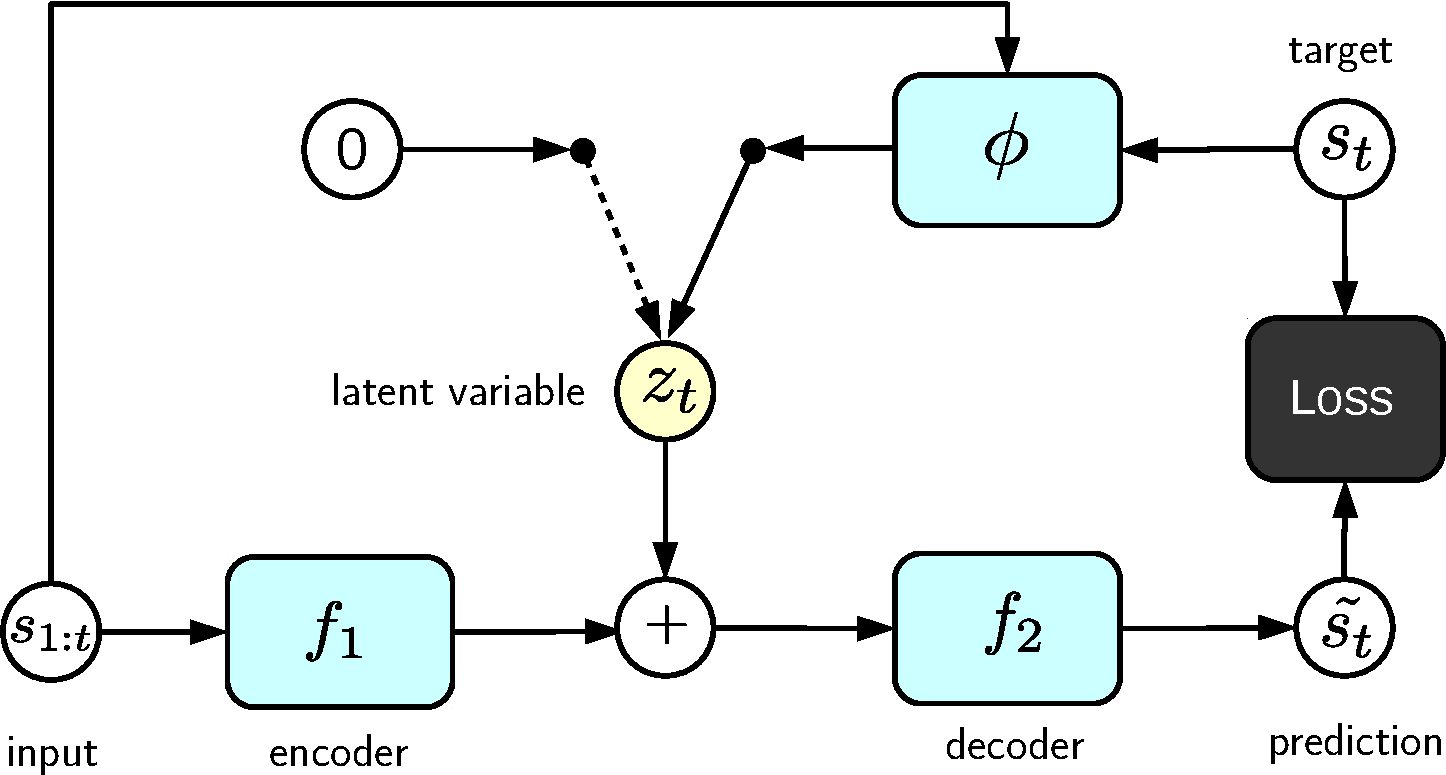
\includegraphics[width=0.5\textwidth]{images/ae_train-crop.pdf}
  \caption{
    \textbf{Target-Encoding Network diagram.}
  }
\end{figure}

Our stochastic prediction model can be viewed as a conditional autoencoder paired with a non-parametric  or semi-parametric sampling procedure.
The architecture consists of three neural networks: an encoder $f_\text{enc}$, a decoder $f_\text{dec}$, and a latent variable network $f_\phi$.
For each input $s_{1:t}$ (\emph{i.e.}\ a sequence of $t$ consecutive states) and a target $s_{t+1}$ (\emph{i.e.}\ the following state), the update equations are given by:
%
\begin{align}
  \label{eq:update-eqn}
  z_t &= f_\phi(s_{1:t}, s_{t+1}) \cdot u, u \in \{0, 1\} \sim \mathcal{B}(p) \\
  \hat{s}_{t+1} &= f_\text{dec}(f_\text{enc}(s_{1:t}), z_t) = f_\theta(s_{1:t}, z_t)
\end{align}
%
where $z_t$ is the latent variable vector associated to the input $s_{1:t}$, $\hat{s}_{t + 1}$ is the reconstructed target state, and $\mathcal{B}(p)$ is a Bernoulli random variable with probability $p$.
All networks are trained by gradient descent to optimize the following objective:
%
\begin{align}
  \ell(\hat{s}_{t+1}, s_{t+1}) &= \lVert \hat{s}_{t+1} - s_{t+1} \rVert_2^2 \\
  &= \lVert f_\theta(s_{1:t}, f_\phi(s_{1:t}, s_{t+1}) \cdot u) - s_{t+1} \rVert_2^2 \doteq J(\theta, \phi)
\end{align}

Note in particular that no sampling or reparamaterization is done at training time.
In standard autoencoders, some mechanism is used to limit the information content of the latent representation to avoid learning trivial mappings and thus encourage the model to learn good representations.
In the conditional case we are considering, we also need such a mechanism to prevent the network from simply reconstructing $s_{t+1}$ from $z_t$ while ignoring the input $s_{1:t}$.
This is accomplished by setting the latent vector $z_t$ to zero with some probability $1 - p$ at every training iteration.
This setting encourages the network to continue to extract as much information as possible from the input $s_{1:t}$, rather than simply trying to reconstruct the target, and only use the true target $s_{t+1}$ to reconstruct what cannot be predicted from the input.
In our experiments, we train with $p = 0$ for an initial fixed number of iterations, which corresponds to purely deterministic training, after which we increase $p$ to incorporate the latent variables encoded from the targets.

A second key point is that the dimension of the latent variable $z$ is much lower than the dimension of the state $s$.
This has two benefits: first, it can further help limit the information content and prevent trivial reconstructions of the targets.
Second, it allows us to use non-parametric estimates of the distribution over latent variables using a reasonable number of points, which we detail in the next section.
A transformation $f_\text{exp}$ transforms this low-dimensional latent variable to be the same size as the hidden representation, after which it is combined via addition.
Note that in the case of a linear transformation, this simply corresponds to combining the latent variable and hidden state via concatenation.

%In our experiments we found setting the dimension of $z$ to be of much lower dimension than $s$ to work well, however other methods, such as adding a sparsity or contractive penalty term, could also be used.

\begin{minipage}[t]{7cm}
  \vspace{0pt}

  \begin{algorithm}[H]
    \caption{Build Stochastic Model}
    \begin{algorithmic}[1]
      \State \textbf{input} training set $\mathcal{D}$
      \State initialize networks $f_\theta, f_\phi$
      \While{not converged}
      \State sample a sequence $\{s_1, \;\cdots, s_{t+1}\} \sim \mathcal{D}$
      \State $z_t = f_{\phi}(s_{1:t}, s_{t+1}) \cdot u$
      \State $\hat{s}_{t+1} = f_{\theta}(s_{1:t}, z_t)$
      \State $J(\theta, \phi) = \|\hat{s}_{t+1} - s_{t+1} \|_2^2$
      \State $\theta \leftarrow \theta - \eta \nabla_\theta J$
      \State $\phi \leftarrow \phi - \eta \nabla_\phi J$
      \EndWhile
      \State $\mathcal{Z} \leftarrow \varnothing$
      \For{$n = 1:N$}
      \State sample a sequence $\{s_1, \;\cdots, s_{t+1}\} \sim \mathcal{D}$
      \State $z_t = f_{\phi}(s_{1:t}, s_{t+1})$
      \State $\mathcal{Z} \leftarrow \mathcal{Z} \cup \{ z_t \}$
      \EndFor
      \State \textbf{return} $f_\theta, \mathcal{Z}$
      %\State
    \end{algorithmic}
  \end{algorithm}
\end{minipage}%
\begin{minipage}[t]{7cm}
  \vspace{0pt}

  \begin{algorithm}[H]
    \caption{Sampling Procedures}\label{algo-sample}
    \begin{algorithmic}[1]
      \Procedure{SampleUniform}{$\mathcal{Z}$}
      \State sample $z \sim \mathcal{Z}$ uniformly at random
      \State \textbf{return} $z$
      \EndProcedure

      \Procedure{KNN}{$\mathcal{Z}, z, k$}
      \State $\mathcal{S} \gets $ set of $k$ nearest neighbors of $z$ in $\mathcal{Z}$
      \State \textbf{return} $\mathcal{S}$
      \EndProcedure

      \Procedure{SampleKNN}{$\mathcal{Z}, z, k$}
      \State $\mathcal{S} \gets \textsc{KNN}(\mathcal{Z}, z, k)$
      \State $z \gets \textsc{SampleUniform}(\mathcal{S})$
      \State \textbf{return} $z$
      \EndProcedure

      \Procedure{SampleMDN}{$\mathcal{Z}, f_\psi, s_{1:t}$}
      \State $(\bm{\tau}, \bm{\mu}, \bm{\sigma}) = f_\psi(s_{1:t})$
      \State $z^* \sim \mbox{GMM}(\bm{\tau}, \bm{\mu}, \bm{\sigma})$
      \State $z \gets \textsc{SampleKNN}(\mathcal{Z}, z^*, 1)$
      \State \textbf{return} $z$
      \EndProcedure
    \end{algorithmic}
    \vspace{5.7pt}
  \end{algorithm}
\end{minipage}

\begin{comment}
  \begin{algorithm}[t]
    \caption{Build Stochastic Model}\label{algo-train}
    \begin{algorithmic}[1]
      \State \textbf{Input} Training set $\mathcal{D}$.
      \State Initialize networks $f_\theta, f_\phi$
      \While{not converged} \Comment{Train networks}
      \State Sample a sequence $\{s_1, ..., s_t, s_{t+1}\} \sim \mathcal{D}$
      \State $z_t = f_{\phi}(s_{1:t}, s_{t+1})$
      \State $\hat{s}_{t+1} = f_{\theta}(s_{1:t}, z_t)$
      \State $\ell(\theta, \phi) = \|s_{t+1} - \hat{s}_{t+1} \|_2^2$
      \State $\theta \leftarrow \theta - \eta \nabla \theta$
      \State $\phi \leftarrow \phi - \eta \nabla \phi$
      \EndWhile
      \State $\mathcal{Z} \leftarrow \varnothing$     \Comment{Estimate latent distribution}
      \For{$i = 1:N_Z$}
      \State Sample a sequence $\{s_1, ..., s_t, s_{t+1}\} \sim \mathcal{D}$
      \State $z_t = f_{\phi}(s_{1:t}, s_{t+1})$
      \State $\mathcal{Z} \leftarrow \mathcal{Z} \cup \{ z_t \}$
      \EndFor
      \Return $f_\theta, \mathcal{Z}$
    \end{algorithmic}
  \end{algorithm}
\end{comment}

\subsection{Sampling} \label{sec:sampling}

After the model is trained, we need a sampling scheme to pair latent variables $z$ with novel input sequences $s_{1:t}$ for which we want to generate future states.
Since we do not use any prior on the latent distribution during training, we cannot assume the latent distribution follows a known parametric form which we can sample from.
Instead, we obtain a non-parametric estimate of the distribution over latent vectors by extracting a large collection of $z$ vectors from the training set, which we refer to as $\mathcal{Z}$.
We explore three sampling methods based on this estimate, which are described explicitly in \cref{algo-sample}.

%Our sampling scheme is based on ideas from manifold learning, for which there is an extensive literature \citep{isomap, LLE, Belkin2003, TSNE}.
%These methods assume we are given a set of points $\{x_i\}$ which are assumed to lie on a low-dimensional manifold $\mathcal{M}$, and approximate the manifold by forming a graph whose vertices are $\{x_i\}$ and whose edges (which can be weighted or unweighted) depend on the Euclidean distance between them.
%In particular, two points are connected by an edge if they are close in Euclidean distance, as this approximates the geodesic distance along the manifold as it becomes small.
%Paths along the manifold can then be approximated by paths along the graph, and it can be shown that given a sufficiently dense sampling of points, graph distances converge to geodesic distances \citep{Bernstein2000}.

%Our sampling scheme is based on such ideas, in particular, we can treat the vectors $z$, extracted from the training set, as points sampled from the unknown latent manifold, form a graph approximation to this manifold using these points, and sample trajectories on this manifold to generate new trajectories in the original input space.

%After training, we extract all vectors $z$ from the training set and use these as inputs to the stochastic prediction model.

\textbf{Uniform} \quad
For a given input $s_{1:t}$, we simply sample some $z \sim \mathcal{Z}$ uniformly at random, in this case the latent variable is independent of the input.

\textbf{\emph{k}-Nearest Neighbors (KNN)} \quad
Here we make a smoothness assumption on the trajectories followed along the latent manifold.
In particular, we assume that $z_{t+1}$ tends to be closer (on average) to $z_t$ than a random other vector in $\mathcal{Z}$.
This assumption is motivated by a smoothness assumption on the inputs: if $s_{t+1}$ and $s_{t+2}$ are close and $f_\phi$ is a smooth function, then $z_t$ and $z_{t+1}$ will be close as well.
This smoothness assumption can be reflected by restricting the choice of $z_{t+1}$ we sample from $\mathcal{Z}$ to the $k$-nearest neighbors of $z_t$.
This approach can be implemented by constructing a $k$-nearest neighbor graph and performing a random walk along this graph.

\textbf{Mixture Density Network (MDN)} \quad
We can also learn an input-dependent prior by training a neural network to assign likelihood values to different vectors in $\mathcal{Z}$ for a given input $s_{1:t}$.
Specifically, we train an MDN \citep{mixture-density-networks} $f_\psi(s_{1:t})$ which outputs the parameters $(\bm{\tau}, \bm{\mu}, \bm{\Sigma})$ of a Gaussian mixture model (with diagonal covariances) and is trained to maximize the likelihood of $z_t$ given $s_{1:t}$ under this model.
Note that Gaussian mixture models can approximate arbitrary distributions given a sufficient number of components, hence this is not a conceptual limitation to the class of prior distributions that can be represented with our approach.

%Although they offer increased flexibility, non-parametric approaches to modeling distributions can also bring potential challenges, which we discuss here.
One potential challenge with using non-parametric approaches to modeling distributions is that the memory and computational cost can increase with the number of points used to construct the estimate, \emph{i.e.}\ $\mathcal{Z}$.
We provide a discussion in \cref{computational-cost}.
In our experiments, we found that the cost of exact nearest neighbor searches required by the last two sampling schemes was lower than the cost of forward passes through other parts of the network, hence this did not pose a limitation.

%A possible issue in modeling distributions using non-parametric approaches is that they can trade flexibility for increased memory and computational cost.

\begin{comment}
  \begin{algorithm}[t]
    \caption{Sampling Procedures}\label{algo-sample}
    \begin{algorithmic}[1]

      \Procedure{KNN}{$\mathcal{Z}, z, K$}
      \State $\mathcal{S} \gets $ set of $K$ nearest neighbors of $z$ in $\mathcal{Z}$.
      \State \textbf{return} $\mathcal{S}$
      \EndProcedure

      \Procedure{SampleUniform}{$\mathcal{Z}$}
      \State Sample $z \sim \mathcal{Z}$ uniformly at random
      \State \textbf{return} $z$
      \EndProcedure

      \Procedure{SampleKNN}{$\mathcal{Z}, z, K$}
      \State $\mathcal{S} \gets \textsc{KNN}(\mathcal{Z}, z, K)$
      \State $z \gets \textsc{SampleUniform}(\mathcal{S})$
      \State \textbf{return} $z$
      \EndProcedure

      \Procedure{SampleLearnedPrior}{$\mathcal{Z}, f_\psi, s_{1:t}$}
      \State $(\pi, \mu, \sigma) = f_\psi(s_{1:t})$
      \State $z^* \sim \mbox{GMM}(\pi, \mu, \sigma)$
      \State $\{z\} \gets \textsc{KNN}(\mathcal{Z}, z^*, 1)$
      \State \textbf{return} $z$
      \EndProcedure
    \end{algorithmic}
  \end{algorithm}
\end{comment}

\section{Related Work}

In recent years, several works have explored prediction of complex time series such as video \citep{mathieu-iclr-2016,canziani2017cortexnet, VPN}.
These typically train models to predict future frames with the goal of learning good representations which disentangle factor of variation and can be used for unsupervised learning \citep{Srivastava15, Villegas17, DentonB17} or learn action-conditional forward models which can be used for planning \citep{Oh15, FinnGL16, Poke, VPN}.
Several works have included latent variables as a means to model the uncertainty, using the framework of Variational Autoencoders \citep{Babaeizadeh2018, Denton2018} (VAEs).
In contrast to VAEs, our model does not place any priors on the latent variable distribution, which removes the need for an additional loss term enforcing consistency between the prior and posterior.
Additionally, our approach does not require any sampling at training time which reduces the variance in the gradients.

Our model is related to Gated and Relational Autoencoders \citep{RelationalAE, GAE}, which were used to learn transformations between pairs of images in an unsupervised manner.
The general architecture and loss is similar in both our works, however their focus was on representation learning for static images while ours is on video generation, and they do not consider sampling schemes for generation.

Our model is also related to Generative Latent Optimization \citep{GLO}, which assigns one latent variable per training sample; latent variables are optimized through gradient descent.
Our method computes latent variables using a learned parametric function, and we also investigate sampling schemes at generation time.
Also related to our method is the Vector-Quantized VAE \citep{VQVAE} (VQ-VAE), where the latent variable is discrete.
Our model could be seen as a form of VQ-VAE where the are as many discrete latent variables as there are training samples.

\section{Data sets}

%In addition to evaluating our method on existing data sets used in the literature, we also use a new, large-scale data set for training and evaluating deep predictive models.
The Next Generation SIMulation program's Interstate 80 (NGSIM I-80) freeway data set \cite{halkias2006ngsim} captures 3 segments of 15 minutes each of a 0.5 km long section of the eastbound I-80 in the San Francisco Bay area in Emeryville in 2005.
Seven cameras, mounted on the top of a 30-story building, record a segment of highway including 6 lanes and an onramp with a frame rate of $10\,\text{Hz}$.
A viewpoint transformation is applied to rectify the perspective, and each vehicle entering the interested section is classified (type), characterised (size), localised (global and local coordinates), and therefore tracked (coordinates over frame count) for its whole journey, totalling over all 5.5k distinct trajectories and 4.5M individual entries.

Our use of this data set is motivated by two main factors.
First, it can potentially allow us to learn predictive models of driver behavior, which have important applications for autonomous driving.
An autonomous vehicle equipped with an accurate predictive model of its surroundings can potentially anticipate unsafe situations and alert the driver.
A predictive model can also be used for model-based planning, and can be learned from observational data without interacting with the environment.

Second, this data set reflects complex interactions between a large number of agents (in this case vehicle drivers), leading to a challenging prediction problem which can be useful for evaluating new methods more generally.
Current video prediction data sets used in the literature to evaluate stochastic prediction models consist of Synthetic Moving MNIST (SM-NIST) digits \citep{Denton2018}, BAIR robot manipulation videos \citep{Ebert17}, or videos of human movements \citep{Denton2018, Babaeizadeh2018}.
These have the advantage of being able to evaluate specific model capabilities in a controlled setting, and have applications in robotics.
However, they also have relatively few degrees of freedom: \emph{e.g.}\ the SM-MNIST data set latent variables are two-dimensional (vertical and horizontal random velocities are picked), while the major factors of variation within the BAIR robot data set can also be captured with two dimensions \textcolor{red}{(\emph{i.e.}\ the position or velocity of the robot arm, which we demonstrate in our experiments)}.
In contrast, the NGSIM I-80 data set has a relatively large number of cars per context image, as shown in \cref{car-statistics}, with each car having multiple degrees of freedom.
We therefore believe this prediction tasks offers unique features which complement other data sets used in the literature.

\begin{figure}
  \centering
  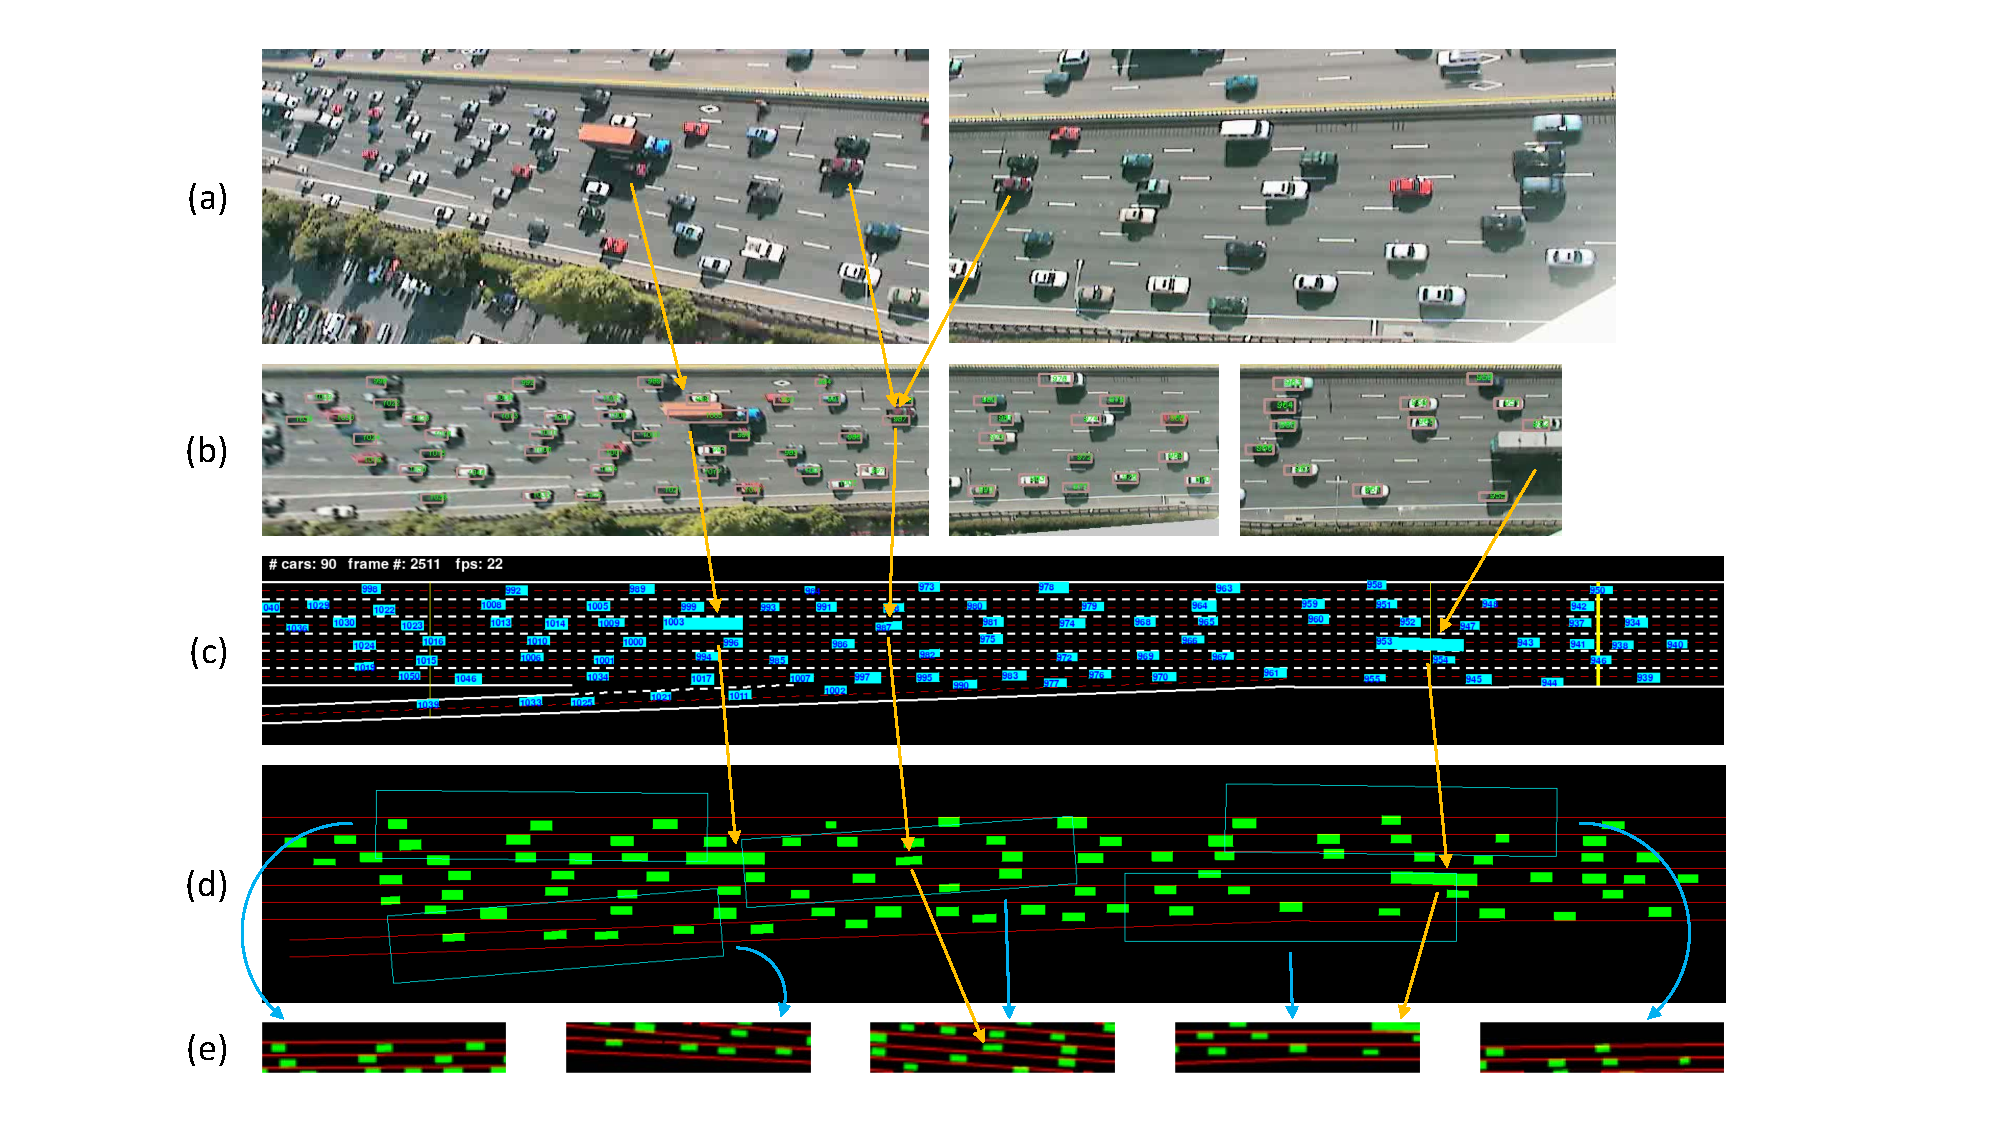
\includegraphics[width=\textwidth]{images/I-80}
  \caption{
    \textbf{Preprocessing pipeline for the NGSIM-I80 data set.}
    \textcolor{Orange}{Orange arrows} show same vehicles across stages.
    \textcolor{ProcessBlue}{Blue arrows} show corresponding extracted context state.
    \textbf{(a)} Snapshots from two of the seven cameras.
    \textbf{(b)} View point transformation, car localisation, characterisation, classification, and tracking.
    \textbf{(c)} Every vehicle in the simulator is initialised with starting position, initial velocity, dimensions, and ID number.
    At every time step, we use the tracked trajectories and a simplified kinematic model of a car to compute the agent actions $(a, b)$, corresponding to acceleration and tangential deviation.
    The vehicle internal state is then updated with one step of the Euler method.
    %    A longitudinal and transverse inter-vehicle linear proximity cost is computed, which is maximum in case of collision and goes to zero if vehicles are sufficiently spaced.
    Finally, the vehicles are drawn onto the screen canvas and displayed with their corresponding ID number.
    \textbf{(d)} Lanes and vehicles are also drawn on a secondary canvas, from which the context states are extracted.
    Rectangular regions around each vehicle constitute the context states.
    %    At this stage, the lane-crossing cost is computed using a modified morphological distance transform between each vehicle and the lane channel.
    \textbf{(e)} Five examples of context states extracted at the previous stage.
    Notice how vehicles oriented slightly to the left (2nd and 3rd examples) have lane markings rotated to the right.
  }
\end{figure}

\section{Experiments}

We now describe our experimental results on two real-world data sets.
We also encourage the reader to view videos at \url{https://sites.google.com/view/targetencodingnetworks/home}.

\subsection{BAIR Results}

The BAIR robot pushing data set \citep{Ebert17} consists of videos of a Sawyer robotic arm randomly moving objects on a table.
The data set contains a high degree of stochasticity due to the random arm motion, and also contains real-world objects and backgrounds.
Following previous work \citep{Babaeizadeh2018, Denton2018}, we condition our model on the first two frames in a video sequence and train it to predict the following 10 frames.
We used the same model architecture as in \citep{Denton2018}, to isolate factors and better understand the influence of our loss and sampling procedure (details can be found in \cref{bair-details}.
The main difference is that we did not use a prior network at training time, did not include a KL term in the loss function, and instead sampled latents at test time using the approaches described in \cref{sec:sampling}.
We also used a lower-dimensional latent variable, with 2 rather than 32 dimensions as in \citep{Denton2018}.

\begin{figure}
  \centering
  \begin{subfigure}[b]{0.49 \textwidth}
    \includegraphics[width=0.49\textwidth]{images/bair_tenet_comparison_ssim-crop.pdf}
    \includegraphics[width=0.49\textwidth]{images/bair_tenet_comparison_psnr-crop.pdf}
    \caption{}
  \end{subfigure}
  \begin{subfigure}[b]{0.49 \textwidth}
    \includegraphics[width=0.49\textwidth]{images/bair_all_comparison_ssim-crop.pdf}
    \includegraphics[width=0.49\textwidth]{images/bair_all_comparison_psnr-crop.pdf}
    \caption{}
  \end{subfigure}
  \caption{
    \textbf{Best-of-$k$ performance on the BAIR data set.}
    The best PSNR and SSIM out of 100 generated samples compared to the test sample is reported.
    Shading indicates $95\%$ confidence interval.
    \textbf{(a)} Comparison between different TENet latent variable sampling schemes: uniform, $k$-nearest neighbors or using a learned Mixture Density Network.
    \textbf{(b)} Comparison to VAE-based approaches.
  }
  \label{bair}
\end{figure}

\begin{figure}
  \centering
  \centering
  \includegraphics[width=0.8\textwidth]{images/robot_trajectory-crop.pdf}
  \caption{
    \textbf{Trajectory generated on the BAIR data set.}
    Top images are generated frames, bottom images show the latent 2-D codes extracted from the training set.
    The code sampled at each time step is marked in red.
  }
  \label{robot-trajectory}
\end{figure}

We follow the evaluation protocol used in previous works on stochastic generation \citep{Walker2016, Babaeizadeh2018, Denton2018}, where we generate a fixed number of samples (in this case 100) using the stochastic model, compare each sample to the ground truth sample in the test set, and report the error of the best match.
We refet to this metric in the rest of the paper as the ``best-of-$k$'' metric.
This method provides some measure of how well the stochastic model covers the space of possible futures, although it does not necessarily reflect the realism of all the generated samples.
Results using both PSNR and SSIM \citep{SSIM} as a metric are shown in \cref{bair}.

We see that all TENet variants outperform the deterministic baseline.
The KNN variant performs better than the uniform, supporting the smoothness assumption that underlies it, and the MDN version with the learned prior network performs best of all.
Compared to variational-based approaches, TENet-MDN performs best for the first few predicted timesteps according to both SSIM and PSNR, and for predictions further into the future the performance of TENet-MDN, TENet-KNN and \textcolor{red}{SVG-MDN becomes statistically equivalent.}
Interestingly, the relative performance of \citep{Babaeizadeh2018} depends on the performance metric.
The fact that our model is able to achieve performance which is similar or better than other state-of-the-art approaches using a latent variable with only two dimensions suggests that this data set is in fact quite simple.
Please refer to the URL for videos.

\subsection{NGSIM-I80 Dataset}

We next report results on the NGSIM-I80 Dataset.
Here we again compared our TENet architecture to a VAE-based model with an identical architecture except for the different loss function and sampling procedure.
%We conditioned the model on sequences of 10 initial states, provided it a sequence of 20 actions and trained it to predict the subsequent 20 states corresponding to those actions.
%This corresponds to a setting where the model is required to evaluate different candidate action sequences by generating predictions corresponding to those actions.
We used an autoregressive model taking 10 consecutive states as input and producing a prediction for the next state as well as a cost at the following timestep.
The predicted state is then concatenated with the 9 previous states and input back into the model, and this procedure is repeated 19 times, resulting in 20 predicted states which are compared to the ground truth states to produce a loss.
Further details of the loss and architecture used can be found in \cref{sec:NGSIM-details}.

Results using the best-of-$k$ metric are shown in \cref{best-of-k-i80}.
Sampling using the KNN scheme offers a significant improvement over the uniform sampling, while using the learned prior network improves performance further, outperforming both the deterministic and VAE models for the first few time steps.
We note an interesting phenomenon: for time steps further into the future, the performance of the deterministic model improves relative to the stochastic models according to the best-of-$k$ metric.
It eventually even performs \emph{better}, even though it is clear from visual inspection that the deterministic predictions are actually becoming worse further into the future.
We provide an explanation of this in \cref{proof}, along with a proof that the best-of-$k$ metric does indeed favor a deterministic averaging model over an exact model as the number of futures gets large in the case of a simple uniform distribution over one-hot vectors.
This is evidence that the best-of-$k$ metric should be interpreted with caution when the number of possible futures becomes large.
In particular, this number can grow exponentially with the number of time steps into the future which are predicted.

\begin{figure}[t!]
  \begin{minipage}[t]{0.49 \textwidth}
    \centering
    \includegraphics[width=\textwidth]{images/comparison_all_i80}
    \caption{
      \textbf{Best-of-$k$ performance on the NGSIM-I80 data set.}
      The best PSNR out of 200 generated samples compared to the test sample is reported.
      Shading indicates $95\%$ confidence interval.
    }
    \label{best-of-k-i80}
  \end{minipage} \quad%
  \begin{minipage}[t]{0.49 \textwidth}
    \centering
    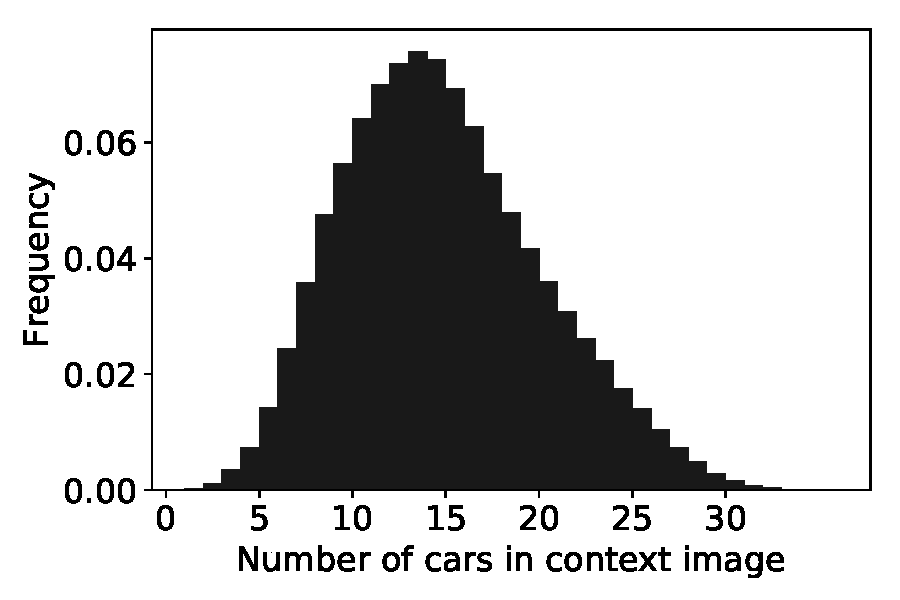
\includegraphics[width=\textwidth]{images/car_statistics}
    \caption{
      \textbf{Cars per context state.}
      Most of the time there are 13 vehicles in the context state, and at most 30.
    }
    \label{car-statistics}
  \end{minipage}
\end{figure}

\begin{table}[t!]
  \caption{
    \textbf{Quantitative performace on NGSIM-I80.}
    Scores assigned by a critic independently trained to classify real samples from samples generated by the different models on the NGSIM-I80 data set, averaged over 20 random seeds.
    $p$-value indicates whether the difference between cVAE and TENet-MDN scores is statistically significant according to a Wilcoxon rank-sum test.
  }
  \label{critic-table}
  \centering
  \begin{tabular}{l|l|lll}
    \toprule
    Training iteration     & Deterministic & cVAE & TENet-MDN & $p$-value \\
    \midrule
    500 & 0.00951 & 0.10296 & 0.11437 & 0.2134 \\
    1000 & 0.00183 & 0.00989 & \textbf{0.02681} & 0.0284 \\
    1500 & 0.00095 & 0.00168 & \textbf{0.00391} & 0.0068 \\
    2000 & 0.00059 & 0.00074 & \textbf{0.00154} & 0.0002 \\
    \bottomrule
  \end{tabular}
\end{table}

\begin{figure}[t!]
  \centering
  \includegraphics[width=\textwidth]{images/qualitative_I-80}
  \caption{
    \textbf{Predicted states visual comparison $\tau$-times-steps in the future.}
    Four alternative futures $\hat{s}_{t+(1:\tau)}$ are visualised and compared.
    Multiple frames are shown using the \emph{ghost} function $g(x_{t+(1:\tau)})$, which superimpose 3 frames 5 time steps apart, backwards, starting from the last one $t + \tau$, where $\tau = 15 = 1.5\,\text{s}$.
    \textbf{Left:} each of the four images is the ghost function corresponding to the $k$-th future prediction, generated with the sequence of latent variable $z_{1:\tau}^{(k)}$.
    \textbf{Centre, black box:} ghost function of the true future $s_{t+(1:\tau)}$.
    \textbf{Right:} differential images between predictions  and ground truth (GT) $\tau$-time-steps in the future.
    %\textbf{Right:} differential images between predictions (\textcolor{LimeGreen}{green vehicle} and \textcolor{OrangeRed}{red lanes}) and ground truth (GT, \textcolor{Mulberry}{purple vehicles} and \textcolor{PineGreen}{dark green lanes}) $\tau$-time-steps in the future.
    \textcolor{Dandelion}{\textbf{Orange box:}} the predicted vehicle (\textcolor{LimeGreen}{green}) is much ahead than GT (\textcolor{Mulberry}{purple}).
    \textcolor{ProcessBlue}{\textbf{Blue box:}} in future 1 the two vehicles (\textcolor{LimeGreen}{green}) move in opposite relative direction wrt GT (\textcolor{Mulberry}{purple}), in future 2 both vehicles (\textcolor{LimeGreen}{green}) are slower than GT (\textcolor{Mulberry}{purple}).
    \textcolor{Red}{\textbf{Red boxes:}} the ego car, turning to the right, makes appear \textcolor{OrangeRed}{red}-\textcolor{PineGreen}{green} lanes on the top, and \textcolor{PineGreen}{green}-\textcolor{OrangeRed}{red} lanes on the bottom.
    \textcolor{LimeGreen}{\textbf{Green box:}} a new car (\textcolor{LimeGreen}{green}) appears in the context state.
    }
    \label{I-80_qual}
\end{figure}

Since we are also interested in measuring the ability of models to generate predictions over long time horizons, we provide a complementary measure where we train a separate classifier to distinguish between real and generated images after the stochastic model has been trained.
This approach has been used in several works to evaluate GANs \citep{Danihelka17, Rosca17, GANeval}, however it is applicable to generative models more broadly.
After the critic is trained to classify real from generated sequences (conditioned on initial sequences drawn from the training set), we use it to produce predictions for sequences generated by conditioning on initial sequences drawn from the testing set.
We use the critic predictions as scores to evaluate the quality of generated sequences, \textcolor{red}{which corresponds to the GC criterion in \citep{GANeval}.}
Details of this training procedure and scoring can be found in \cref{critic-details}.

Resulting scores are shown in \cref{critic-table}.
The deterministic model has the lowest score, the VAE has a higher score, which agrees with its improved perceptual quality, and the TENet-MDN has the highest.
This provides further evidence that it is able to generate high-quality predictions far into the future.

\section{Conclusion}

In this work we have made two contributions towards research in stochastic prediction: a new model architecture which is simple to train and does not suffer from mode collapse or posterior mismatch, and a challenging large-scale data set with real-world applications in autonomous driving.
We will make this data set publicly available to the research community in an effort to encourage more research in this area.
In future work, we plan to apply our stochastic forward model for model-based planning under uncertainty, by back-propagating gradient of predicted costs with respect to input actions.
%Our preparation of this data set also makes it straightforward to use for planning, by having agents execute actions which are rendered in the simulator.

%\subsection{Figures}
%
%
%
%\subsection{Tables}
%
%
%\begin{table}
%  \caption{Sample table title}
%  \label{sample-table}
%  \centering
%  \begin{tabular}{lll}
%    \toprule
%    \multicolumn{2}{c}{Part}                   \\
%    \cmidrule(r){1-2}
%    Name     & Description     & Size ($\mu$m) \\
%    \midrule
%    Dendrite & Input terminal  & $\sim$100     \\
%    Axon     & Output terminal & $\sim$10      \\
%    Soma     & Cell body       & up to $10^6$  \\
%    \bottomrule
%  \end{tabular}
%\end{table}
%
%\section{Final instructions}

% \subsubsection*{Acknowledgments}
%
% Use unnumbered third level headings for the acknowledgments. All
% acknowledgments go at the end of the paper. Do not include
% acknowledgments in the anonymized submission, only in the final paper.

\newpage

\bibliographystyle{unsrt}
\bibliography{nips_2018}

\newpage

\begin{appendices}
  \crefalias{subsection}{appsec}
  \section{Appendix}

  \subsection{Algorithm Details}

  \begin{minipage}[t]{7cm}
    \vspace{0pt}

    \begin{algorithm}[H]
      \caption{Train Prior Network}
      \begin{algorithmic}[1]
        \State Initialize Mixture Density Network $f_\psi$
        \While{not converged}
        \State Sample a sequence $\{s_1, ..., s_t, s_{t+1}\} \sim \mathcal{D}$
        \State $(\bm{\tau}, \bm{\mu}, \bm{\Sigma}) = f_{\psi}(s_{1:t})$
        \State $z_t = f_{\phi}(s_{1:t}, s_{t+1})$
        %    \State $\mathcal{L}_\text{MDN} = $
        \State $\mathcal{L}_\text{MDN} = \text{pdf}_\text{GMM}(z_t | \bm{\tau}, \bm{\mu}, \bm{\Sigma})$\footnotemark
        \State $\psi \gets \psi - \eta \nabla \mathcal{L}_\text{MDN}$
        \EndWhile
      \end{algorithmic}
    \end{algorithm}
  \end{minipage}%
  \begin{minipage}[t]{7cm}
    \vspace{0pt}

    \begin{algorithm}[H]
      \caption{Generate Sequence}\label{algo-sample}
      \begin{algorithmic}[1]
        \State \textbf{Input} Initial sequence $s_{1:t}$, $\mathcal{Z}$.
        \For{j = 1:T}
        \State $z \gets \textsc{Sample}(\mathcal{Z})$
        \State $s_{t+j} = f_\theta(s_{1:(t+j-1)}, z)$
        \EndFor
        \Return $s_{1:(t+T)}$
        \State
        \State
        \State
        \State
      \end{algorithmic}
    \end{algorithm}
  \end{minipage}
  \footnotetext{this refers to the likelihood of $z_t$ under a Gaussian mixture model with parameters $(\bm{\tau}, \bm{\mu}, \bm{\Sigma})$, \emph{i.e.}\ $\text{pdf}_\text{GMM}(z_t | \bm{\tau}, \bm{\mu}, \bm{\Sigma}) = \sum_i \tau_i \frac{1}{\sqrt{(2\pi)^k |\Sigma_i|}} \text{exp}\Big[-(z_t - \mu_i)^\top\Sigma_i^{-1}(z_t - \mu_i)\Big]$}

  \subsection{Details for BAIR Experiments} \label{sec:BAIR-details}
  \label{bair-details}

  This architecture consists of a VGG16 frame encoder and decoder combined with a 2-layer LSTM network with 128 hidden units.
  Our models were trained using ADAM \citep{ADAM} with a learning rate of 0.002.
  For the TENet we also set the dimension of $z$ to be lower (2 dimensions) and trained the model with dropout parameter $p = 0$ on the latent code (corresponding to purely deterministic mode) until the loss stopped decreasing, after which we set $p = 0.5$.

  \subsection{Details for NGSIM-I80 Dataset Experiments} \label{sec:NGSIM-details}

  We first give some additional data set details.
  After preprocessing, at every time step we have the following items for each car in the video frame:

  \begin{itemize}
    \item A context image $i_t$ of size $2 \times 120 \times 24$, capturing lane and neighboring car information
    \item A 4-dimensional vector $p_t$ encoding the car's position and velocity
    \item A 2-dimensional action $a_t$ encoding the car's acceleration and change in angle
    \item A 2-dimensional cost vector $c_t$ encoding two different cost functions: one reflecting its proximity to other cars and a second its overlap with lanes.
  \end{itemize}

  The state $s_t$ at a given time step is a list $(i_t, p_t)$.
  In addition to predicting the future state, models are also trained to predict future costs.
  The per-timestep prediction loss which all the models optimize is given by:

  \begin{equation}
    \ell(\hat{s}_t, s_t) = \|\hat{i}_t - i_t \|_2^2 + \| \hat{p}_t - p_t \|_2^2 + \| \hat{c}_t - c_t \|_2^2
  \end{equation}

  The architectural components used by the models are listed in the table below.

  \begin{table}[h]
    \caption{Architecture Details for NGSIM-I80 experiments}
    \label{sample-table}
    \centering
    \begin{tabular}{lll}
      \toprule
      Network & Sub-Networks     & Architecture    \\
      \midrule
      \multirow{3}{*}{$f_\text{enc}$} & Image Encoder & 3-layer convnet with 128 feature maps, reshaped output size 5376 \\
      & State Encoder & 2-layer MLP with 128 hidden units, size 4-128-128-5376 \\
      & Action Encoder & 2-layer MLP with 128 hidden units, size 2-128-128-5376  \\
      \hline
      \multirow{3}{*}{$f_\text{dec}$} & Image Decoder & 3-layer deconvnet with 128 feature maps \\
      & State Decoder & 2-layer MLP with 128 hidden units, size 5376-128-128-4 \\
      & Cost Predictor & 2-layer MLP with 128 hidden units, size 5376-128-128-1 \\
      \hline
      $f_\phi$ & Frame Encoder & 3-layer convnet with 128 feature maps followed by 2-layer MLP \\ & & with 128 hidden units, size 5376-128-128-$|z|$ (for TENet) \\
      &               & or 5376-128-128 (for VTENet) \\
      \hline
      $f_\text{exp}$ & Expansion Network & 2-layer MLP with 128 hidden units, size $|z|$-128-128-5376\\
      \hline
      \bottomrule
    \end{tabular}
  \end{table}

  The deterministic model only uses $f_\text{enc}$ and $f_\text{dec}$.
  For the TENet, $f_\phi$ represents the network in \cref{eq:update-eqn}.
  For the VAE, $f_\phi$ represent the posterior network and outputs the parameters $(\mu, \sigma)$ of a diagonal Gaussian which the latent vector $z$ is sampled from.
  All models are trained with ADAM \citep{ADAM} using a learning rate of 0.0001.
  The TENet and VAE models have their encoder and decoder initialized with the encoder and decoder of the deterministic model to speed up training, and both have a latent code size of $|z|=32$.
  The TENet is trained to optimize the loss $\ell(s_t, \hat{s}_t)$.
  The VAE additionally includes a KL term and is trained to minimize the following loss:

  \begin{equation}
    \ell_{\text{VAE}} = \ell(s_t, \hat{s_t}) + \beta \cdot \mbox{KL}(\mathcal{N}(0, I), \mathcal{N}(\mu, \sigma))
  \end{equation}

  We optimized the $\beta$ parameter over the range $\{1, 0.1, 0.01, 0.001, 0.0001, 0.00001 \}$ in an initial search, and found that values greater than $0.0001$ yielded image predictions which resembled those of the baseline model.
  We therefore used $0.0001$ in subsequent experiments.

  \begin{table}
    \caption{NGSIM-I80 data set statistics}
    \label{i80-stats}
    \centering
    \begin{tabular}{ll}
      \toprule
      Training Sequences     & 10454 \\
      Validation Sequences & 579 \\
      Testing Sequences & 579 \\
      Average Sequence Length & 348.7 \\
      \bottomrule
    \end{tabular}
  \end{table}

  \subsection{A note on evaluation} \label{proof}

  We provide a discussion of evaluation metrics, and their relationship to the stochasticity of the prediction task.
  Here we argue that the best-of-$k$ metric used in previous work \citep{Walker2016, Babaeizadeh2018, Denton2018} becomes less meaningful as the number of possible futures becomes large.
  Consider the task of modeling a distribution of one-hot vectors, where each sample is a binary vector with all zeros except for a single $1$, whose index is chosen uniformly between $1$ and $n$.
  A baseline model which always predicts the average $\hat{y} = (1/n, 1/n, ..., 1/n)$ (which is clearly not a valid sample in the target distribution) will have an expected loss of $\sqrt{(n-1)/n}$.
  A stochastic model which exactly captures the true distribution will have an expected loss of $\sqrt{2} \cdot F(k, k, (n-1)/n)$, where $F$ refers to the cumulative distribution function of a Binomial random variable with $p = (n-1)/n$ (proofs can be found in the Appendix).
  Curves of both of these loss functions for different $n$ are shown in \cref{expected-loss}.
  These illustrate that as $n$ becomes large, an increasingly high number of samples is required for the correct stochastic prediction model to outperform the deterministic baseline according to this metric.

  The baseline model always produces the same prediction $\hat{y} = (\frac{1}{n}, ..., \frac{1}{n})$.
  Each sample from the true distribution is of the form $y_i = (0, ..., 0, 1, 0, ..., 0)$ with a single non-zero element.
  \begin{align}
    \mathbb{E}[\mathcal{L}_{\mbox{baseline}}] &= \sqrt{\sum_{i=1}^n (\hat{y}_i - y_i)^2} \\
    &= \sqrt{(1-\frac{1}{n})^2 + (n-1)\Big ( \frac{1}{n} \Big )^2} \\
    &= \sqrt{\frac{(n-1)^2 + (n-1)}{n^2}} \\
    &= \sqrt{\frac{n-1}{n}}
  \end{align}

  To compute the best-of-$k$ loss, the true stochastic model produces $k$ samples of the same form as the one drawn from the true distribution, \emph{i.e.}\ $\hat{y}_k = (0, ..., 0, 1, 0, ..., 0)$, where the non-zero index is chosen uniformly from $1$ to $n$.
  Let $j$ denote the non-zero index of the sample drawn from the true distribution and $i_1, i_2, ..., i_k$ non-zero indices of the samples output by the stochastic model.
  The probability of each sample \emph{not} matching $y_j$ is equal to $p = \frac{n-1}{n}$.
  Therefore, the probability of none of the generated samples matching $y_j$ is equal to the cumulative distribution function of a binomial random variable $B(k, p)$, denoted $F(k, k, p)$.
  In the case of a generated sample matching $y_j$, the best-of-$k$ loss will equal 0, otherwise it will equal $\sqrt{2}$.

  Putting this together, the expected best-of-$k$ loss is given by:

  \begin{align}
    \mathbb{E}[\mathcal{L}_{\mbox{best-of-$k$}}] &= \mbox{P(at least one sample matches)}\cdot 0 + \mbox{P(none of the samples match)} \cdot \sqrt{2} \\
    &= \sqrt{2} \cdot F\Big (k, k, \frac{n-1}{n} \Big) \\
  \end{align}

  \begin{figure}
    \centering
    \begin{subfigure}[b]{0.3\textwidth}
      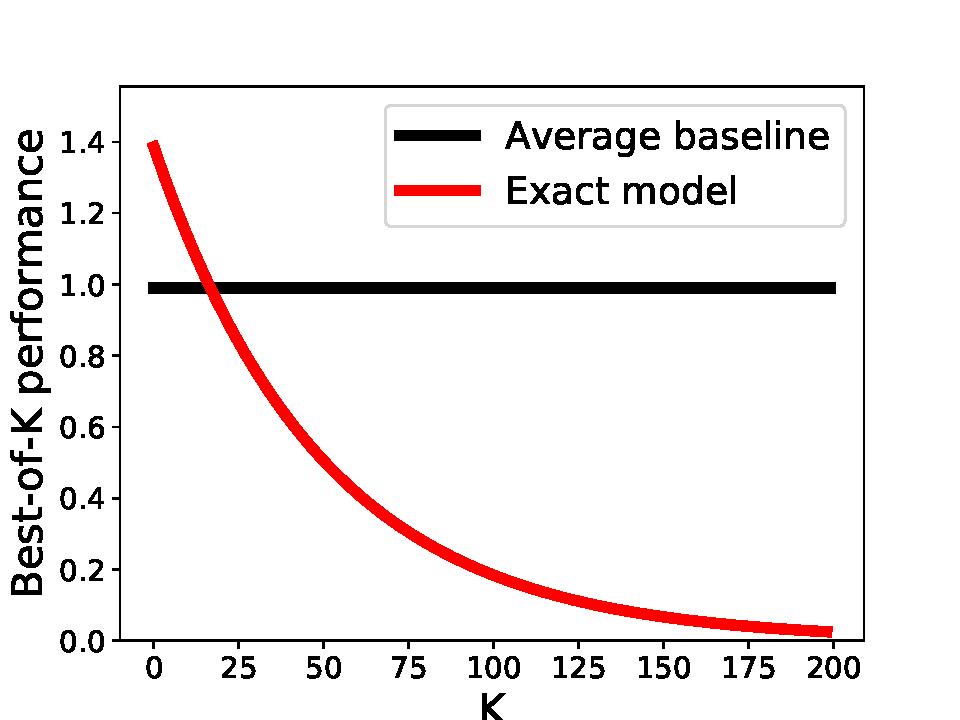
\includegraphics[width=\textwidth]{images/best_of_k_toy_n50.pdf}
      \caption{$n=50$}
      \label{fig:gull}
    \end{subfigure}
    ~ %add desired spacing between images, e. g. ~, \quad, \qquad, \hfill etc.
    %(or a blank line to force the subfigure onto a new line)
    \begin{subfigure}[b]{0.3\textwidth}
      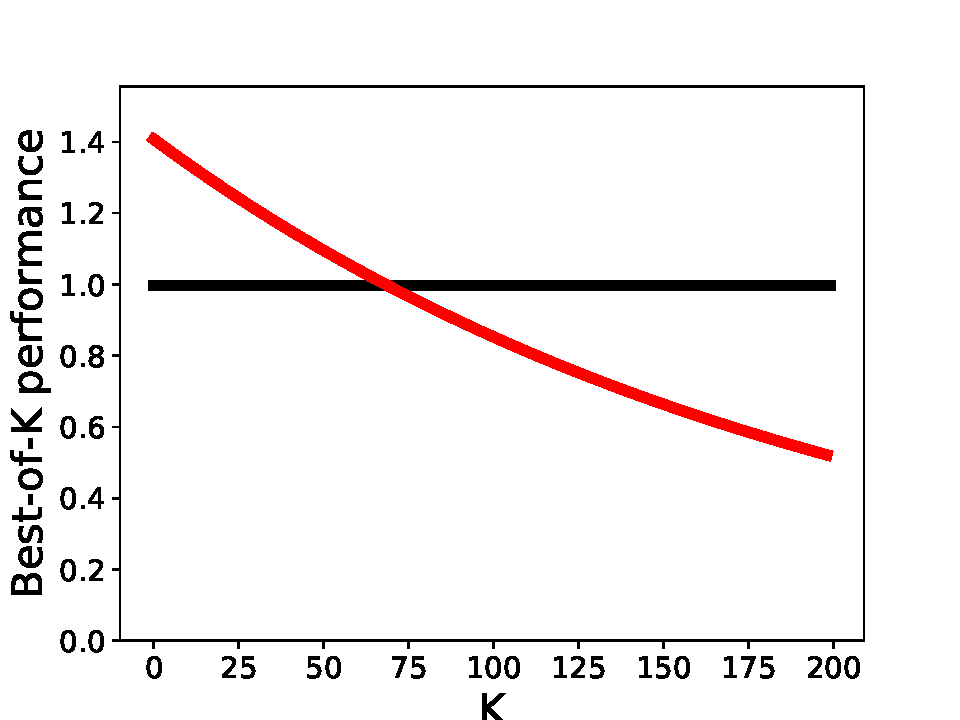
\includegraphics[width=\textwidth]{images/best_of_k_toy_n200.pdf}
      \caption{$n=200$}
      \label{fig:tiger}
    \end{subfigure}
    ~ %add desired spacing between images, e. g. ~, \quad, \qquad, \hfill etc.
    %(or a blank line to force the subfigure onto a new line)
    \begin{subfigure}[b]{0.3\textwidth}
      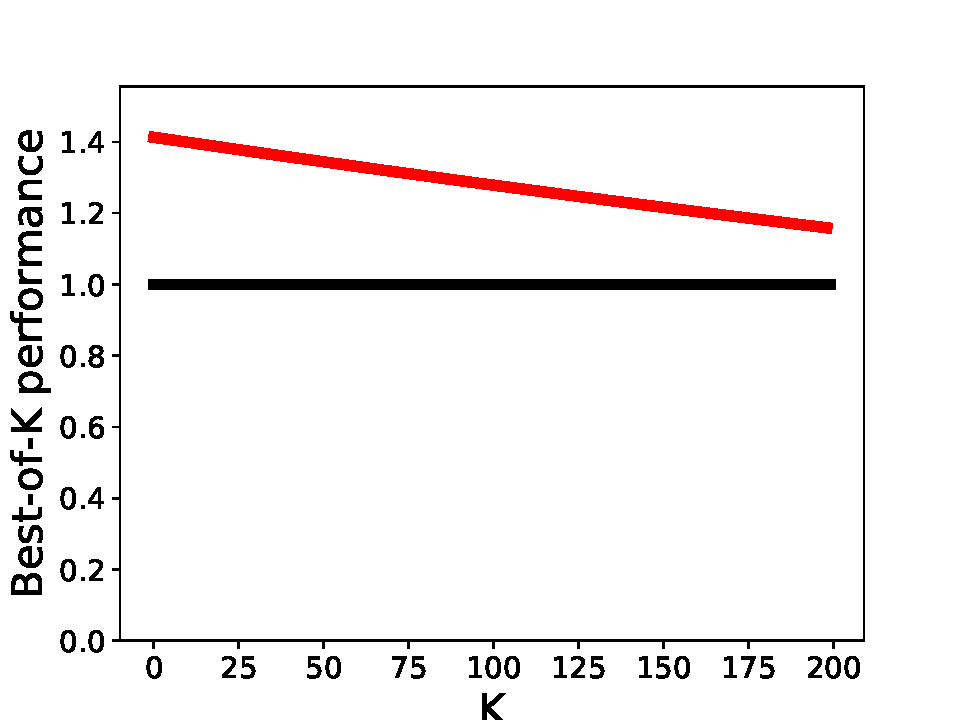
\includegraphics[width=\textwidth]{images/best_of_k_toy_n1000.pdf}
      \caption{$n=1000$}
      \label{fig:mouse}
    \end{subfigure}
    \caption{
      \textbf{Best-of-$k$ performance of average baseline model and true model for different numbers of possible futures $n$.}
      As the number of futures increases, it becomes increasingly difficult for the true model to outperform the baseline according to this metric.}
    \label{expected-loss}
  \end{figure}

  \subsection{Critic Evaluation Details}
  \label{critic-details}

  To help control for factors of variation inherent in the stochastic optimization process of training the critic (such as the order in which samples are presented, weight initialization and gradient noise due to small minibatches), we train the critic on all three models we wish to evaluate (deterministic, cVAE and TENet) jointly.
  More specifically, we construct minibatches where the negatively labeled sequences are produced by the three generative models in equal proportion, and the positively labeled sequences are drawn from the training set.
  The critic is trained on this binary classification problem, and after training produces scores for each of the three generative models.
  This process is described explicitly in \cref{algo-critic}.

  \begin{algorithm}[h]
    \caption{Compare Generative Models using an Offline Critic}\label{algo-critic}
    \begin{algorithmic}[1]
      \State \textbf{Input} Trained generative models $M_1, M_2, ..., M_{N_{models}}$ we wish to evaluate.
      \State Initialize critic model $f_{critic}$
      \For{$j = 1:N_{train}$}
      \State Sample a sequence $\{s_1, ..., s_T\}$ from the training set.
      \State $\mathcal{B} \gets \{\}$ \Comment{Initialize minibatch}
      \State $\mathcal{B}[1] \gets \{s_{t+1}, ..., s_T\}$ \Comment{True Sequence}
      \For{$i = 1:N_{models}$}
      \State $\mathcal{B}[i+1] \gets \textsc{Generate}(M_i, \{s_1, ..., s_t\})$ \Comment{Sequence generated by model $M_i$}
      \EndFor
      \State $p \gets [ ]$
      \For{$i = 1:(N+1)$}
      \State $p[i] \gets f_{critic}(\mathcal{B}[i])$ \Comment{Compute critic predictions}
      \EndFor
      \State $t \gets [1, 0, 0, ..., 0]$ \Comment{True/False labels}
      \State $\mathcal{L}_{critic} \gets $ BinaryCrossEntropy($p, t$)
      \State $f_{critic} \gets f_{critic} - \eta \nabla{\mathcal{L}_{critic}}$
      \EndFor
      \State $S\gets []$ \Comment{Initialize model scores}
      \For{$j = 1:N_{test}$}
      \State Sample a sequence $\{s_1, ..., s_T\}$ from the testing set.
      \For{$i = 1:N_{models}$} \Comment{Score sequence generated by each model}
      \State $S[i] \gets S[i] + f_{critic}(\textsc{Generate}(M_i, \{s_1, ..., s_t\}))$
      \EndFor
      \State $S \gets S / N_{test}$
      \EndFor
      \Return $S$ \Comment{Return model scores}
    \end{algorithmic}
  \end{algorithm}

  \subsection{Timing of Nearest Neighbor Search}
  \label{computational-cost}

  All the approaches above have a memory footprint which grows with the size of $\mathcal{Z}$.
  In terms of computational cost, the first approach requires $\mathcal{O}(1)$ at inference time as we are simply sampling from $\mathcal{Z}$.
  The second approach allows us to construct the nearest-neighbor graph offline, since it is input-independent, hence sampling is also $\mathcal{O}(1)$ at runtime.
  The third approach is input-dependent, and can be cast as a nearest-neighbor problem by first sampling a point from the Gaussian mixture model output by $f_\psi$, and then mapping it to the nearest vector in $\mathcal{Z}$.
  In practice, we found that the computational cost of an exact nearest neighbor search over $\mathcal{Z}$ on GPU was small compared to the cost of forward passes through other parts of the network (see \cref{nn-search-timing}).
  If additional speedups are required, we note that finding nearest neighbors is a well-studied problem for which fast exact or approximate algorithms exist, such as $k$-d trees or locally sensitive hashing.

  \begin{table}
    \caption{
      Timing for different operations.
      Timing for different operations.
      The number of latent codes searched over is 240000 for BAIR and 100000 for NGSIM-I80.
    }
    \label{nn-search-timing}
    \centering
    \begin{tabular}{lcc}
      \toprule
      Operation     & BAIR [ms] & NGSIM-I80 [ms] \\
      \midrule
      Encoding  & 1.2 & 1.4 \\
      Decoding  & 2.8 & 2.4 \\
      NN search & 0.7 & 0.5 \\
      \bottomrule
    \end{tabular}
  \end{table}

  % \subsection{Additional Video Prediction Results}
  %
  % \begin{figure}
  %   \centering
  %   \includegraphics[width=0.4\textwidth]{images/bair_ae_comparison_ssim-crop.pdf}
  %   \includegraphics[width=0.4\textwidth]{images/bair_ae_comparison_psnr-crop.pdf}
  %   \caption{}
  %   \label{bair}
  % \end{figure}

  \begin{figure}
    \centering
    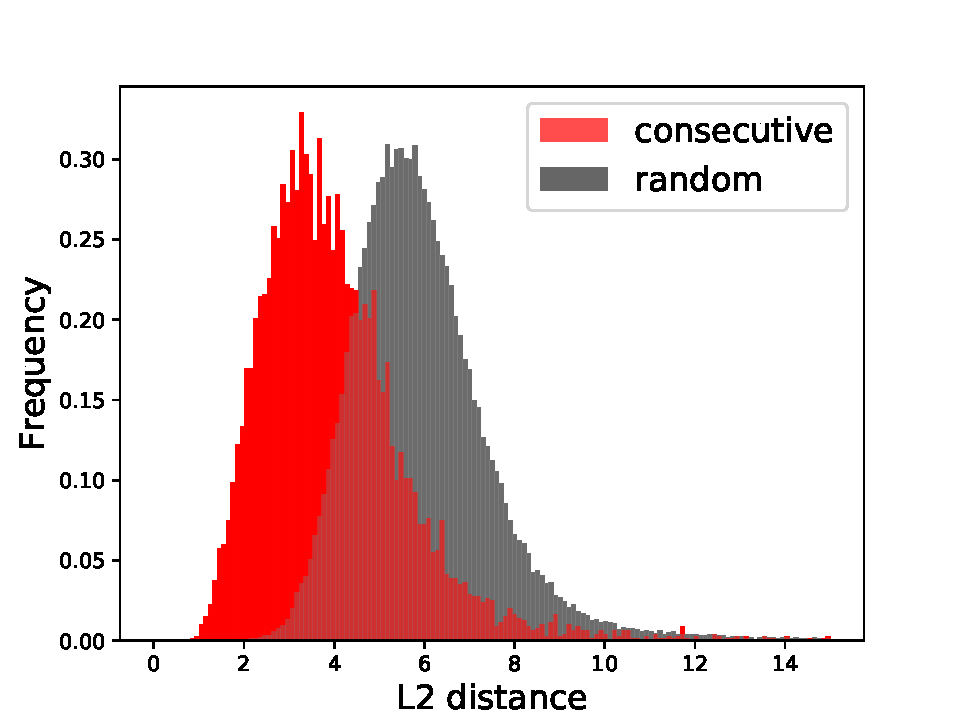
\includegraphics[width=0.5\textwidth]{images/distance_histograms.pdf}
    %  \fbox{\rule[-.5cm]{0cm}{4cm}
    %    \rule[-.5cm]{4cm}{0cm}}
    \caption{
      Distribution of distances between consecutive $z$ and random pairs of $z$ vectors extracted from the I-80 training set.
      Consecutive vectors are closer on average, which supports the smoothness assumption underlying \cref{knn-algo}.
    }
  \end{figure}

  % \section*{References}
  %
  % References follow the acknowledgments. Use unnumbered first-level
  % heading for the references. Any choice of citation style is acceptable
  % as long as you are consistent. It is permissible to reduce the font
  % size to \verb+small+ (9 point) when listing the references. {\bf
  %   Remember that you can use more than eight pages as long as the
  %   additional pages contain \emph{only} cited references.}
  % \medskip
  %
  % \small

\end{appendices}
\end{document}
